\ifx\allfiles\undefined
\documentclass[12pt, a4paper, oneside, UTF8]{ctexbook}
\def\path{../config}
\input{\path/package.tex}

% 定理环境设置
\input{\path/theorem1_zh.tex}

\input{\path/custom.tex}

% 修改参数改变封面样式，0 默认原始封面、内置其他1、2、3种封面样式
\def\myIndex{3}


\ifnum\myIndex>0
    \input{\path/cover_package_\myIndex} 
\fi

\def\myTitle{线性代数笔记}
\def\myAuthor{M.K.}
\def\myDateCover{\today}
\def\myDateForeword{\today}
\def\myForeword{前言}
\def\myForewordText{
    
    这是一个基于\LaTeX{}模板的线代笔记。

}
\def\mySubheading{副标题}


\begin{document}
% \input{\path/cover_text_\myIndex.tex}

\newpage
\thispagestyle{empty}
\begin{center}
    \Huge\textbf{\myForeword}
\end{center}
\myForewordText
\begin{flushright}
    \begin{tabular}{c}
        \myDateForeword
    \end{tabular}
\end{flushright}

\newpage
\pagestyle{plain}
\setcounter{page}{1}
\pagenumbering{Roman}
\pagestyle{fancy}
\fancyfoot[C]{\thepage}
\renewcommand{\headrulewidth}{0.4pt}
\renewcommand{\footrulewidth}{0pt}
\tableofcontents

\newpage
\pagenumbering{arabic}
\setcounter{page}{1}








\else
\fi

\chapter{行列式的计算}
\section{行（列）和相等的情形}
行（列）和相等的情形是行列式计算中常见的一类情形，下面我们通过一个例子来说明如何计算这类行列式．
\begin{align*}D_n &= \begin{vNiceMatrix}[columns-width = auto]
    b & a & a & \cdots & a \\
    a & b & a & \cdots & a \\
    \vdots & \vdots & \vdots & \ddots & \vdots \\
    a & a & a & \cdots & b
\end{vNiceMatrix} 
= \begin{vNiceMatrix}
  b+(n-1)a & a & \cdots & a\\
  b+(n-1)a & a & \cdots & a\\ 
  \vdots & \vdots & \ddots & \vdots \\
  b+(n-1)a & a & \cdots & b  
\end{vNiceMatrix}
=[b+(n-1)a]\begin{vNiceMatrix}[columns-width = auto]
    1 & a & \cdots & a \\
    1 & b & \cdots & a \\
    \vdots & \vdots & \ddots & \vdots \\
    1 & a & \cdots & b
\end{vNiceMatrix}\\[10pt]
&=[b+(n-1)a]\begin{vNiceMatrix}
    1 & 0 & \cdots & 0 \\
    1 & b-a & \cdots & 0 \\
    \vdots & \vdots & \ddots & \vdots \\
    1 & 0 & \cdots & b-a
\end{vNiceMatrix}
=[b+(n-1)a](b-a)^{n-1}
\end{align*}

\section{爪形行列式}
\begin{center}
    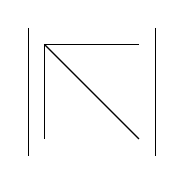
\begin{tikzpicture}[scale=0.3]

\draw[black, line width=0.5pt] (0,0) -- (4,-4);
\draw[black, line width=0.5pt] (0,0) -- (4,0); 
\draw[black, line width=0.5pt] (0,0) -- (0,-4);

% 行列式竖线（可选，如果要表示行列式的话）
\draw[black, line width=0.2pt] (-0.7,0.7) -- (-0.7,-4.7);
\draw[black, line width=0.2pt] (4.7,0.7) -- (4.7,-4.7);

\end{tikzpicture}
\end{center}
爪形行列式结构如图所示．下面我们通过一个例子来说明如何计算这类行列式．\footnote{本文中行列式空白位置均为0，后文同样如此}
\begin{align*}
    D_n &= \begin{vNiceMatrix}[columns-width = 1.8em]
        1 & -1 & -1 & \cdots & -1\\
        1 & a_1\\
        2 & & a_2\\
        \vdots & & & \ddots\\
        n & & & & a_n
    \end{vNiceMatrix}
    \xlongequal{r_1+r_i \times \frac{1}{a_{i+1}},i \ge 2}
    \begin{vNiceMatrix}[columns-width = 1.8em]
        1+\displaystyle\sum_{i=1}^{n}\frac{i}{a_i} & 0 & 0 & \cdots & 0\\
        1 & a_1\\
        2 & & a_2\\
        \vdots & & & \ddots\\
        n & & & & a_n
    \end{vNiceMatrix}\\[10pt]
    &= \left(1+\displaystyle\sum_{i=1}^{n}\frac{i}{a_i}\right)\prod_{i=1}^{n}a_i
\end{align*}
\section{范德蒙德行列式}
\begin{definition}
    形如下面这样的行列式称为范德蒙德行列式
    \[D_n = \begin{vNiceMatrix}[columns-width = 1pt]
    1 & 1 & 1 & \cdots & 1\\
    x_1 & x_2 & x_3 & \cdots & x_n\\
    \vdots & \vdots & \vdots & \ddots & \vdots\\
    x_1^{n-1} & x_2^{n-1} & x_3^{n-1} & \cdots & x_n^{n-1}
\end{vNiceMatrix}
=\prod_{0<i<j\le n}(x_j-x_i)\]
\end{definition}
\begin{example}
    求行列式$D=\begin{vNiceMatrix}
        a & b &c\\
        b+c & a+c & a+b\\
        a^2f & b^2f & c^2f
    \end{vNiceMatrix}$
\end{example}
\begin{solution}
    \[D=\begin{vNiceMatrix}
        a & b &c\\
        b+c & a+c & a+b\\
        a^2f & b^2f & c^2f
    \end{vNiceMatrix}
    =(a+b+c)f\begin{vNiceMatrix}[columns-width = 1.5em]
        a&b&c\\
        1&1&1\\
        a^2&b^2&c^2
    \end{vNiceMatrix}
    =-f(a+b+c)(b-a)(c-a)(c-b)\]
\end{solution}
\section{分块矩阵行列式}
\begin{theorem}
    设$\bm{A}$为$m$阶方阵，$\bm{B}$为$n$阶方阵，$\bm{C}$为$m\times n$或$n\times m$矩阵，则有
    \[\begin{vNiceMatrix}[columns-width = 1.2em]
    \bm{A} & \bm{C}\\
    \bm{0} & \bm{B}
    \end{vNiceMatrix}
    = \begin{vNiceMatrix}[columns-width = 1.2em]
    \bm{A} & \bm{0}\\
    \bm{C} & \bm{B}
    \end{vNiceMatrix}
    = \begin{vNiceMatrix}[columns-width = 1.2em]
    \bm{A} & \bm{0}\\
    \bm{0} & \bm{B}
    \end{vNiceMatrix}
    = |\bm{A}|\cdot |\bm{B}|\]
    \[\begin{vNiceMatrix}[columns-width = 1.2em]
        \bm{C} & \bm{A}\\
        \bm{B} & \bm{0}
    \end{vNiceMatrix}
    =\begin{vNiceMatrix}[columns-width = 1.2em]
        \bm{0} & \bm{A}\\
        \bm{B} & \bm{C}
    \end{vNiceMatrix}
    =\begin{vNiceMatrix}[columns-width = 1.2em]
        \bm{0} & \bm{A}\\
        \bm{B} & \bm{0}
    \end{vNiceMatrix}
    =(-1)^{mn}|\bm{A}|\cdot |\bm{B}|\]
\end{theorem}
\begin{example}
    设$\bm{A},\bm{B}$为2阶方阵，若$|\bm{A}|=2,|\bm{B}|=3$，求
    $\begin{pNiceMatrix}[columns-width = 1.2em]
        \bm{0} & \bm{A}\\
        \bm{B} & \bm{0}
    \end{pNiceMatrix}$的伴随矩阵．
\end{example}
\begin{solution}
    \begin{align*}\begin{pNiceMatrix}[columns-width = 1.2em]
        \bm{0} & \bm{A}\\
        \bm{B} & \bm{0}
    \end{pNiceMatrix}^*
    =\begin{vNiceMatrix}[columns-width = 1.2em]
        \bm{0} & \bm{A}\\
        \bm{B} & \bm{0}
    \end{vNiceMatrix}\cdot
    \begin{pNiceMatrix}[columns-width = 1.2em]
        \bm{0} & \bm{A}\\
        \bm{B} & \bm{0}
    \end{pNiceMatrix}^{-1}
    =|\bm{A}||\bm{B}|
    \begin{pNiceMatrix}[columns-width = 1.2em]
        \bm{0} & \bm{B}^{-1}\\
        \bm{A}^{-1} & \bm{0}
    \end{pNiceMatrix}
    =\begin{pNiceMatrix}[columns-width = 1.2em]
        \bm{0} & 2\bm{B}^*\\
        3\bm{A}^* & \bm{0}
    \end{pNiceMatrix}
\end{align*}
\end{solution}
\section{加边法}
往往对于每行（列）有多次重复出现的数字的行列式，可以通过加边法转换行列式为前面学过的行列式．例如：
\begin{align*}
    &\begin{vNiceMatrix}[columns-width = auto]
        1+a_1 & 1 & 1 & 1 \\
        2 & 2+a_2 & 2 & 2 \\
        3 & 3 & 3+a_3 & 3 \\
        4 & 4 & 4 & 4+a_4
    \end{vNiceMatrix}
    =\begin{vNiceMatrix}[columns-width = auto]
        1 & 0 & 0 & 0 & 0\\
        1 & 1+a_1 & 1 & 1 & 1 \\
        2 & 2 & 2+a_2 & 2 & 2 \\
        3 & 3 & 3 & 3+a_3 & 3 \\
        4 & 4 & 4 & 4 & 4+a_4
    \end{vNiceMatrix}\\
    =&\begin{vNiceMatrix}[columns-width = 1.8em]
        1 & -1 & -1 & -1 & -1 \\
        1 & a_1\\
        2 & & a_2\\
        3 & & & a_3\\
        4 & & & & a_4
    \end{vNiceMatrix}
    =\left(1+\sum_{i=1}^{4}\frac{i}{a_i}\right)\prod_{i=1}^{4}a_i
\end{align*}

\begin{example}
    计算行列式$D_n=\begin{vNiceMatrix}[columns-width = 1.5em]
        b_1+a_1& a_1 & \cdots & a_1\\
        a_2 & b_2+a_2 & \cdots & a_2\\
        \vdots & \vdots & \ddots & \vdots\\
        a_n & a_n & \cdots & b_n+a_n
    \end{vNiceMatrix}$
\end{example}
\begin{solution}
    \[D_n=\begin{vNiceMatrix}[columns-width = 1em]
        1 & 0 & 0 & \cdots & 0\\
        a_1 & b_1+a_1 & a_1 & \cdots & a_1\\
        a_2 & a_2 & b_2+a_2 & \cdots & a_2\\
        \vdots & \vdots & \vdots & \ddots & \vdots\\
        a_n & a_n & a_n & \cdots & b_n+a_n
    \end{vNiceMatrix}
    =\begin{vNiceMatrix}[columns-width = 1.8em]
        1 & -1 & -1 & \cdots & -1\\
        a_1 & b_1\\
        a_2 & & b_2\\
        \vdots & & & \ddots\\
        a_n & & & & b_n
    \end{vNiceMatrix}
    =\left(1+\sum_{i=1}^{n}\frac{a_i}{b_i}\right)\prod_{i=1}^{n}b_i\]
\end{solution}

\section{么形行列式}
\begin{center}
    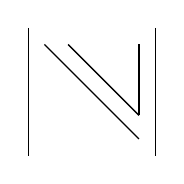
\begin{tikzpicture}[scale=0.3]

\draw[black, line width=0.5pt] (0,0) -- (4,-4);
\draw[black, line width=0.5pt] (1,0) -- (4,-3); 
\draw[black, line width=0.5pt] (4,0) -- (4,-3);

% 行列式竖线（可选，如果要表示行列式的话）
\draw[black, line width=0.2pt] (-0.7,0.7) -- (-0.7,-4.7);
\draw[black, line width=0.2pt] (4.7,0.7) -- (4.7,-4.7);

\end{tikzpicture}
\end{center}
么形行列式结构如图所示，图中只展示了开口朝上的情形，上下左右对称的开口朝下、朝左、朝右的么形行列式结构类似，处理方法相同，均按照开口方向展开．
\begin{example}
    计算行列式$D_n=\begin{vNiceMatrix}[columns-width = 1.8em]
        2 & 0 & \cdots & 0 & 2\\
        -1 & 2 & \cdots & 0 & 2\\
        & -1 & \ddots & \vdots & \vdots\\
        & & \ddots & 2 & 2\\
        & & & -1 & 2
    \end{vNiceMatrix}$
\end{example}
\begin{solution}
    将$D_n$按第一行展开得
    \[D_n=2\begin{vNiceMatrix}[columns-width = 1.8em]
        2 & \cdots & 0 & 2\\
        -1 & \ddots & \vdots & \vdots\\
        & \ddots & 2 & 2\\
        & & -1 & 2
    \end{vNiceMatrix}_{n-1}
    +(-1)^{n+1}2\begin{vNiceMatrix}[columns-width = 1.8em]
        -1 & 2 & \cdots & 0\\
        & -1 & \ddots & \vdots\\
        & & \ddots & 2\\
        & & & -1
    \end{vNiceMatrix}_{n-1}\]
    于是可得
    \[D_n=2D_{n-1}+2(-1)^{n+1}(-1)^{n-1}=2D_{n-1}+2\]
    又$D_1=2$，$D_n + 2=2(D_{n-1}+2)$，解得$D_n=2^{n+1}-2$
\end{solution}

\section{川形行列式}
\begin{center}
    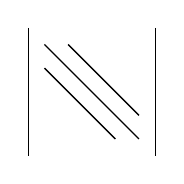
\begin{tikzpicture}[scale=0.3]

\draw[black, line width=0.5pt] (0,0) -- (4,-4);
\draw[black, line width=0.5pt] (1,0) -- (4,-3); 
\draw[black, line width=0.5pt] (0,-1) -- (3,-4);

% 行列式竖线（可选，如果要表示行列式的话）
\draw[black, line width=0.2pt] (-0.7,0.7) -- (-0.7,-4.7);
\draw[black, line width=0.2pt] (4.7,0.7) -- (4.7,-4.7);

\end{tikzpicture}
\end{center}
川形行列式结构如图所示，处理时先按首行展开，再按首列展开，得到递推关系．
\begin{example}
    计算行列式$D_n=\begin{vNiceMatrix}[columns-width = 1.5em]
        2a & 1 &\\
        a^2 & 2a & 1 \\
        & a^2 & 2a & \ddots \\
        & & \ddots & \ddots & 1\\
        & &  & a^2 & 2a
    \end{vNiceMatrix}$
\end{example}
\begin{solution}
    将$D_n$按第一行展开得
    \[D_n=2a\begin{vNiceMatrix}[columns-width = 1.5em]
        2a & 1 \\
        a^2 & 2a & \ddots \\
        & \ddots & \ddots & 1\\
        &  & a^2 & 2a
    \end{vNiceMatrix}_{n-1}
    -\begin{vNiceMatrix}[columns-width = 1.5em]
        a^2 & 1 \\
        & 2a & \ddots \\
        & & \ddots & 1\\
        & & & 2a
    \end{vNiceMatrix}_{n-1}\]
    继续将第二个行列式按第一列展开得
    \[D_n=2aD_{n-1}-a^2\begin{vNiceMatrix}[columns-width = 1.5em]
        2a & 1 \\
        a^2 & 2a & \ddots \\
        & \ddots & \ddots & 1\\
        &  & a^2 & 2a
    \end{vNiceMatrix}_{n-2}
    =2aD_{n-1}-a^2D_{n-2}\]
    又$D_1=2a,D_2=3a^2$，解得$D_n=(n+1)a^n$
\end{solution}
\ifx\allfiles\undefined
\end{document}
\fi